\section{Esercizio 5}

\begin{enumerate}[label=\Alph*.]
	
	\item Nel dropbox del corso sono presenti alcuni files di dati del tipo \texttt{CeBr3\_xx.dat} con \texttt{xx} nome di una sorgente di calibrazione: $\mathrm{Cs}^{137}$, $\mathrm{Co}^{57}$, $\mathrm{Na}^{22}$, $\mathrm{Ba}^{133}$ e $\mathrm{Eu}^{152}$.\\
	I dati sono lo spettro in formato ASCII di un MCA (con 8K canali) per un cristallo di $\mathrm{CeBr}_3$ esposto a varie sorgenti di calibrazione. Istogrammare i vari spettri di multicanale e scrivere un programma per determinare posizione e risoluzione spettrale dei picchi di calibrazione, il più automatizzato possibile.\\
	Si discutano i risultati ottenuti in termini di risoluzione energetica del cristallo e linearità.
	\item Utilizzando gli algoritmi di smoothing illustrati a lezione, provare a vedere se si riesce a migliorare la determinazione spettrale dei picchi spettrali trovati: area, altezza... Discutere i risultati ottenuti. 
	
\end{enumerate}

\[* * * \] \smallskip

\noindent In \figurename~\ref{fig:RAW} sono riportati i grafici dei dati, così come riportati nei file di input relativi all'esposizione del cristallo alle diverse sorgenti (conteggi "grezzi"). Per individuarne in maniera automatizzata i picchi di risonanza si è pensato innanzitutto di dividere il dominio spettrale dell'analizzatore multicanale in sotto-bande sulle quali determinare il massimo assoluto dei conteggi: scegliendo opportunamente la larghezza di queste regioni di ottimizzazione locale si ha buona speranza di individuare un sottoinsieme di canali che includa tutti i bin contenenti le frequenze di risonanza cercate. Naturalmente alcuni dei massimi così individuati saranno solo artefatti della suddivisione operata sulla banda del rivelatore (ad esempio valori al bordo di una sotto-banda in cui lo spettro è monotono) per cui rigettiamo tutti quelli che non soddisfino le condizioni elementari che definiscono un punto stazionario di massimo:

\newcounter{conditions}
\begin{enumerate}
\item derivata prima dei conteggi compresa in un piccolo intorno dello zero;
\item derivata seconda dei conteggi minore di una certa soglia negativa.
\setcounter{conditions}{\value{enumi}}
\end{enumerate}

\noindent A questo punto si saranno certamente individuati dei massimi locali dell'intero spettro che siano anche ottimi globali nelle rispettivi sotto-regioni di ricerca.\\

\noindent Resta tuttavia qualche criticità su eventuali \emph{plateau} degli spettri analizzati: mancando nelle sotto-regioni interessate dei picchi "veri", le oscillazioni riconducibili al rumore intrinseco della rivelazione danno inevitabilmente luogo a \emph{falsi positivi} (ossia massimi locali non associati a risonanze del cristallo scintillatore). Per ovviare a tal problema è stata definita un'ulteriore condizione necessaria per l'accettazione dei valori selezionati:

\begin{enumerate}
	\setcounter{enumi}{\value{conditions}}
	\item  numero di conteggi maggiore di una certa soglia, associabile ai picchi di rumore.
\end{enumerate}

\noindent Naturalmente tutta la difficoltà di implementazione dell'algoritmo risiede nella definizione dei parametri per le condizioni (1), (2) e (3), considerate soprattutto la richiesta di massima automazione della routine e la conseguente sconvenienza di un'accordatura manuale da operare di volta in volta sulla base dei dati analizzati. Si è scelto di far dipendere opportunamente tali parametri dalla sotto-banda di origine del candidato picco e in particolare di~considerare:

\begin{itemize}
	\item[-] << \texttt{a = 1.10 * mean\{Counts on Sub-Region\}} >> come soglia sui conteggi $(\,y > a\,)$;
	\item[-] << \texttt{b = 0.45 * max\{Derivative - Counts on Sub-Region\}} >> come soglia sulla pendenza $(\,|y'|<b\,)$;
	\item[-] << \texttt{c = 0.05 * max\{2ndDerivative - Counts on Sub-Region\}} >> come soglia sulla concavità $(\,y'' < -c\,)$.
\end{itemize}

\noindent Le derivate dei conteggi sono state valutate numericamente per mezzo di differenze finite al secondo ordine, utilizzando la libreria \texttt{numpy.gradient} di~\texttt{Python}\footnote{Documentazione consultabile al seguente link: \href{https://docs.scipy.org/doc/numpy-1.15.0/reference/generated/numpy.gradient.html}{\texttt{https://docs.scipy.org/doc/[...]/numpy.gradient.html}}}.\\

\noindent Infine, per assicurarsi di eliminare qualsiasi artefatto ancora dovuto al particolare partizionamento dello spettro, si è pensato di ripetere l'intera procedura con una differente scelta per la larghezza dei sotto-intervalli e di accettare definitivamente soltanto i candidati picchi individuati da entrambe le istanze della routine. In particolare, definito innanzitutto il range effettivo dei dati considerati (tutti gli spettri hanno una soglia energetica oltre la quale sono sostanzialmente nulli), l'intervallo risultante è stato suddiviso la prima volta in  20 e la seconda in 8 parti uguali, sulle quali sono stati definiti i candidati picchi, poi filtrati secondo le condizioni (1), (2) e (3). Il confronto diretto tra i due \emph{data-set} così ottenuti ha decretato quali candidati accettare come effettivi picchi di risonanza.\\

\noindent  In \figurename~\ref{fig:PeakSearchRaw} sono indicati (\textit{croci arancioni}) i punti che l'algoritmo proposto ha individuato sugli spettri: risulta subito evidente che qualche picco importante non è stato individuato, soprattutto su  Co$^{57}$ e Na$^{22}$. D'altra parte ci riteniamo soddisfatti dal grado di selettività della routine rispetto ai falsi positivi, considerato l'alto livello di rumore presentato da alcuni degli spettri proposti. I dettagli dell'implementazione in \texttt{Python} possono essere consultati nella prima parte del Listato~\ref{list:PeakRoutine}.\\

\noindent Per indagare la risoluzione energetica del cristallo scintillatore abbiamo deciso di analizzare per ogni spettro il Picco Principale (P.P.), inteso come quello relativo alla risonanza che ha prodotto più conteggi sul rivelatore: la strategia è mirata alla minimizzazione dei problemi dovuti al rumore delle misure.\\

\noindent Innanzitutto è stato necessario definire una \texttt{ROI} (\texttt{Region Of Interest}) attorno al P.P. in modo da poter operare un \emph{fitting} parametrico dei conteggi relativi alla sola risonanza considerata. Si è assunto che il picco abbia profilo simil-Gaussiano, al netto di un eventuale fondo da sottrarre opportunamente. In particolare la \texttt{ROI} attorno al picco è stata definita come il \underline{minimo} intorno del punto di massimo tale da soddisfare le seguenti condizioni, scelte in modo da funzionare robustamente per tutti gli spettri proposti:

\begin{align*}
\Bigl|y_\texttt{ROI} - y_\mathrm{max}\Bigr| &\leq \frac{3}{4} \times y_\mathrm{max}, \\
\\
\Bigl|y'_\texttt{ROI}\Bigr| &< 50.
\end{align*}

\noindent Il fondo è stato approssimato al segmento congiungente i due punti spettrali agli estremi della \texttt{ROI}, per mezzo della libreria \texttt{Python} adibita all'interpolazione polinomiale con metodo l.s.~\!(\emph{least squares}): \texttt{numpy.polyfit}\footnote{Documentazione: \href{https://docs.scipy.org/doc/numpy-1.15.0/reference/generated/numpy.polyfit.html}{\texttt{https://docs.scipy.org/doc/[...]/numpy.polyfit.html}}}. Infine anche il fit Gaussiano è stato ottenuto con metodo l.s., ma adoperando la più generica libreria \texttt{scipy.optimize.curve\_fit}\footnote{Documentazione: \href{https://docs.scipy.org/doc/scipy/reference/generated/scipy.optimize.curve_fit.html}{\texttt{https://docs.scipy.org/doc/[...]/scipy.optimize.curve\_fit.html}}} che permette di definire a piacere il modello da adattare ai dati.

\vfill

\noindent A partire dunque dalla definizione:

\vfill

\begin{equation*}
g(x) = A\,\exp\!\left[\frac{-(x-x_0)^2}{2\sigma^2}\right],
\end{equation*}
 
 \vfill
 
\noindent e fornendo al \emph{fitter} i parametri iniziali:

\vfill

\begin{equation*}
A\,\Bigr|^\mathrm{init} = y_\mathrm{max},\quad x_0\,\Bigr|^\mathrm{init} = x_\mathrm{max},\quad \sigma\,\Bigr|^\mathrm{init} = \hat{\sigma}_x(\texttt{DATA}),
\end{equation*}

\vfill

\noindent otteniamo i risultati\footnote{Larghezza del picco $w$ e relativa risoluzione spettrale $w/x_0$ sono calcolate come da standard \texttt{FWHM}. L'area sottesa è stimata in approssimazione triangolare $S\simeq wA/2$. Le incertezze infine sono ricavate dalla matrice di covarianza restituita dal \emph{fitter}} riportati nelle Figure~\ref{fig:PPRawCs137},~\ref{fig:PPRawCo57},~\ref{fig:PPRawNa22},~\ref{fig:PPRawBa133}~e~\ref{fig:PPRawEu152}.\\

\vfill

\begin{sidewaysfigure}
	\centering
	\caption{Istogrammi grezzi dei cinque spettri di calibrazione considerati.}
	\subfloat{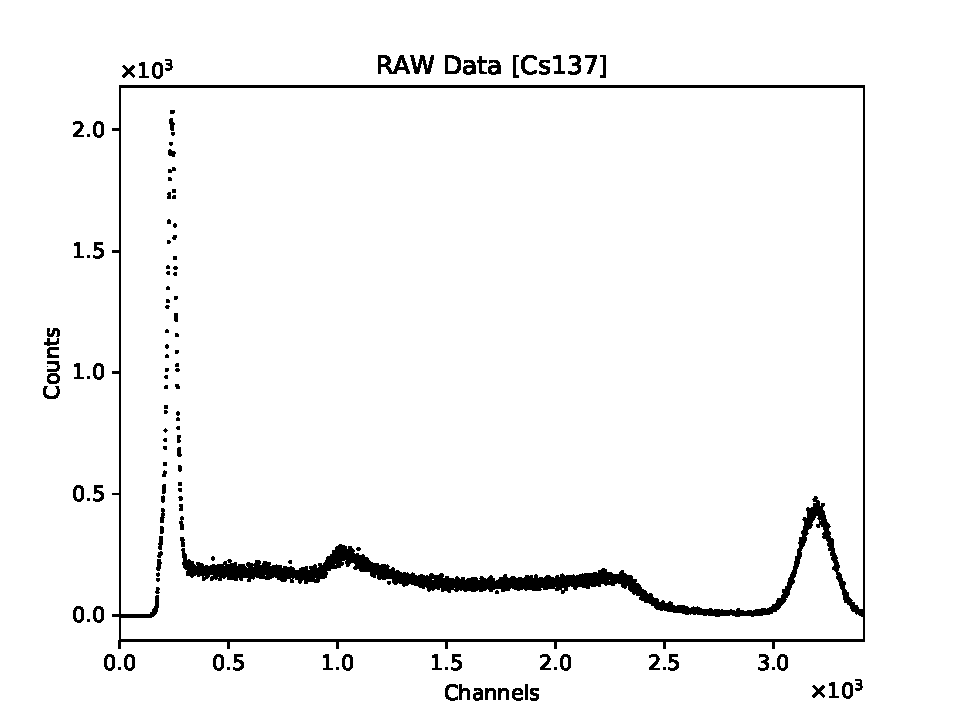
\includegraphics[width = .33\textwidth,trim={.1cm 0 1cm 0}, clip]{Immagini/RawCs137.pdf}} 
	\subfloat{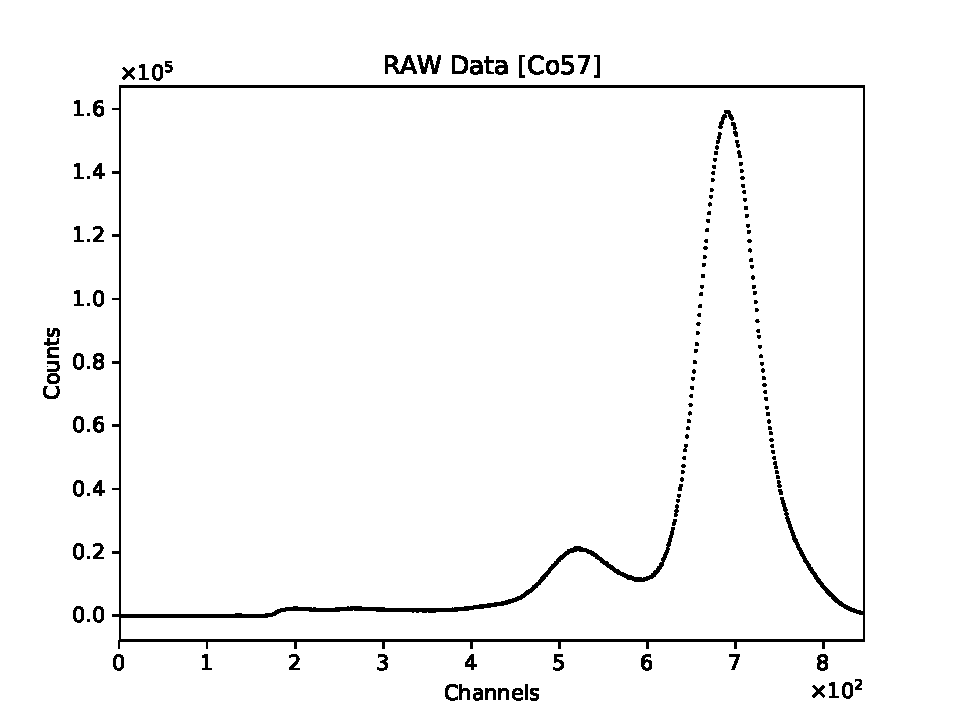
\includegraphics[width =  .33\textwidth,trim={.1cm 0 1cm 0}, clip]{Immagini/RawCo57.pdf}}
	\subfloat{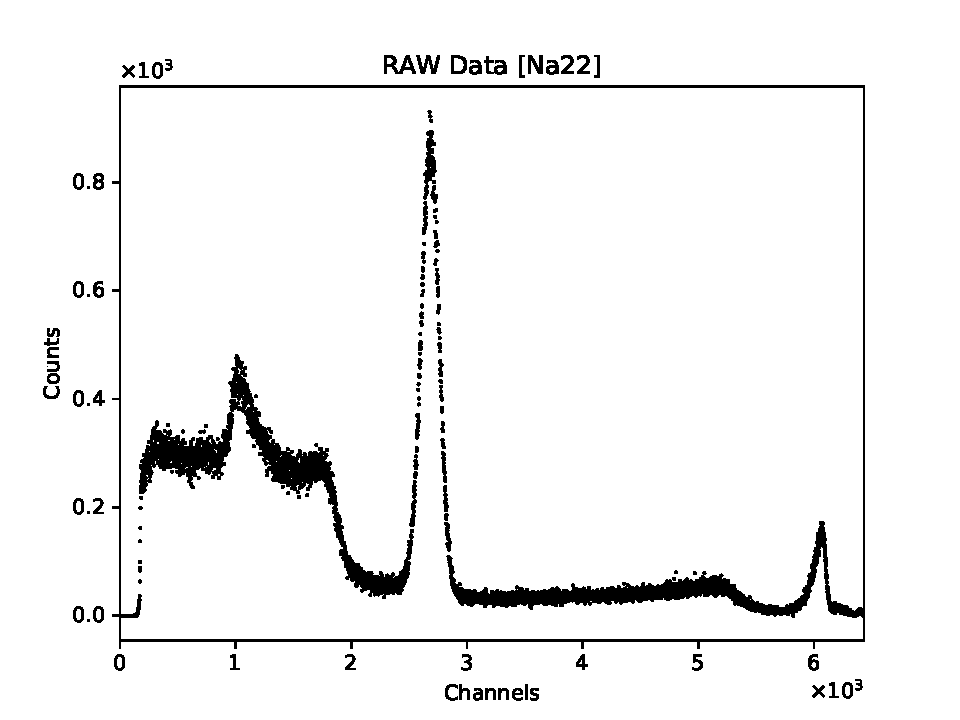
\includegraphics[width = .33\textwidth,trim={.1cm 0 1cm 0}, clip]{Immagini/RawNa22.pdf}}\\
	\subfloat{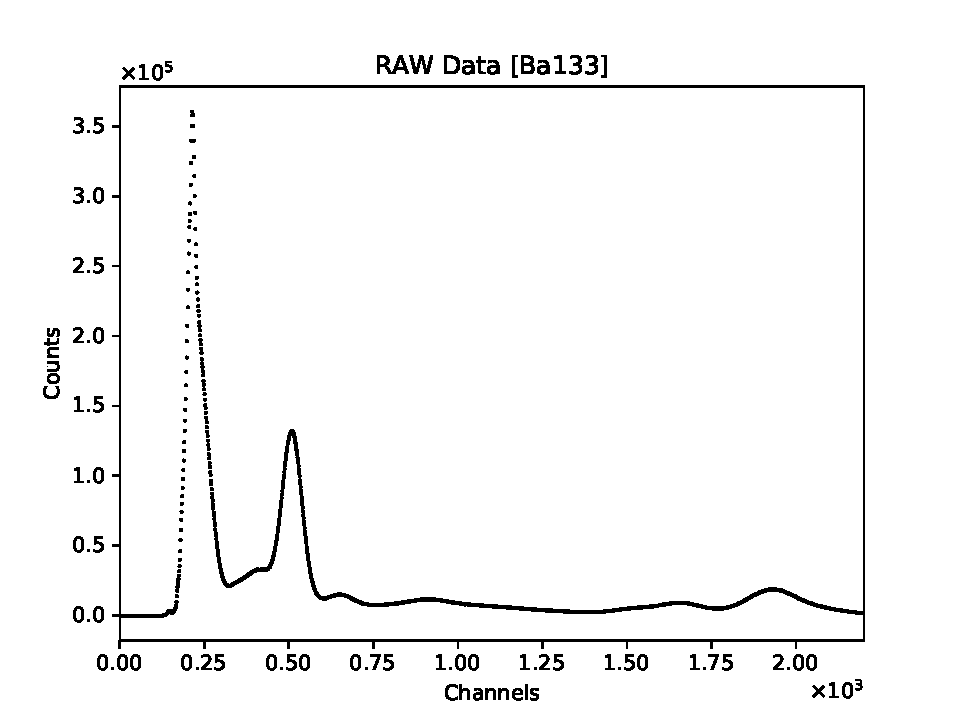
\includegraphics[width = .33\textwidth,trim={.1cm 0 1cm 0}, clip]{Immagini/RawBa133.pdf}}
	\subfloat{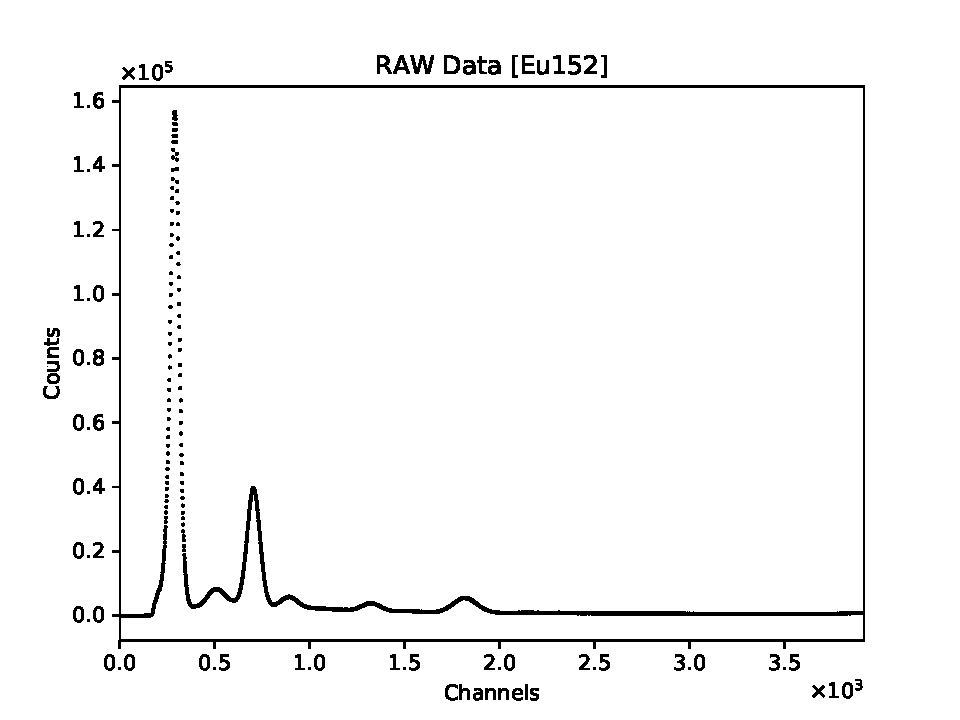
\includegraphics[width = .33\textwidth,trim={.1cm 0 1cm 0}, clip]{Immagini/RawEu152.pdf}}
	\label{fig:RAW}
\end{sidewaysfigure}

\begin{sidewaysfigure}
	\centering
	\caption{Ricerca dei picchi di scintillazione sugli spettri di calibrazione grezzi.}
	\subfloat{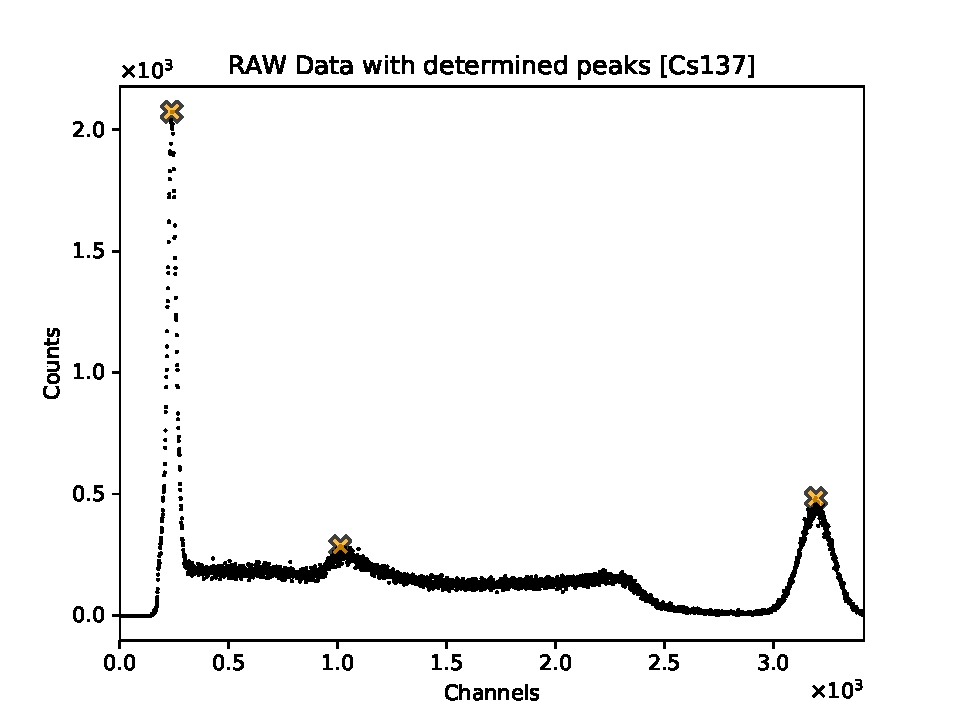
\includegraphics[width = .33\textwidth,trim={.1cm 0 1cm 0}, clip]{Immagini/RawCs137_with_determined_peaks.pdf}} 
	\subfloat{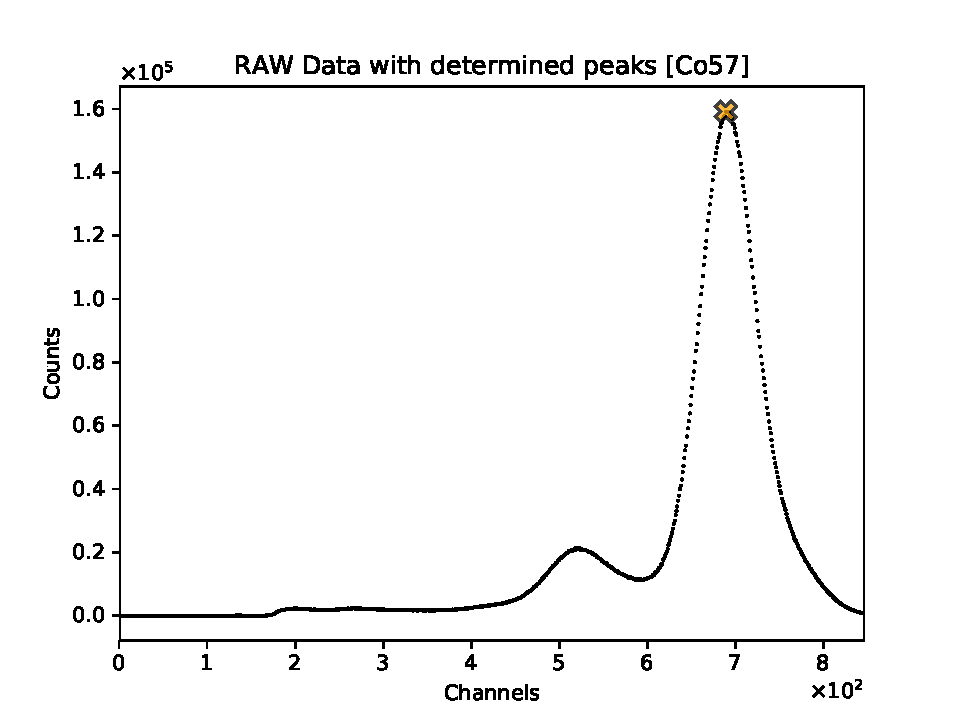
\includegraphics[width =  .33\textwidth,trim={.1cm 0 1cm 0}, clip]{Immagini/RawCo57_with_determined_peaks.pdf}}
	\subfloat{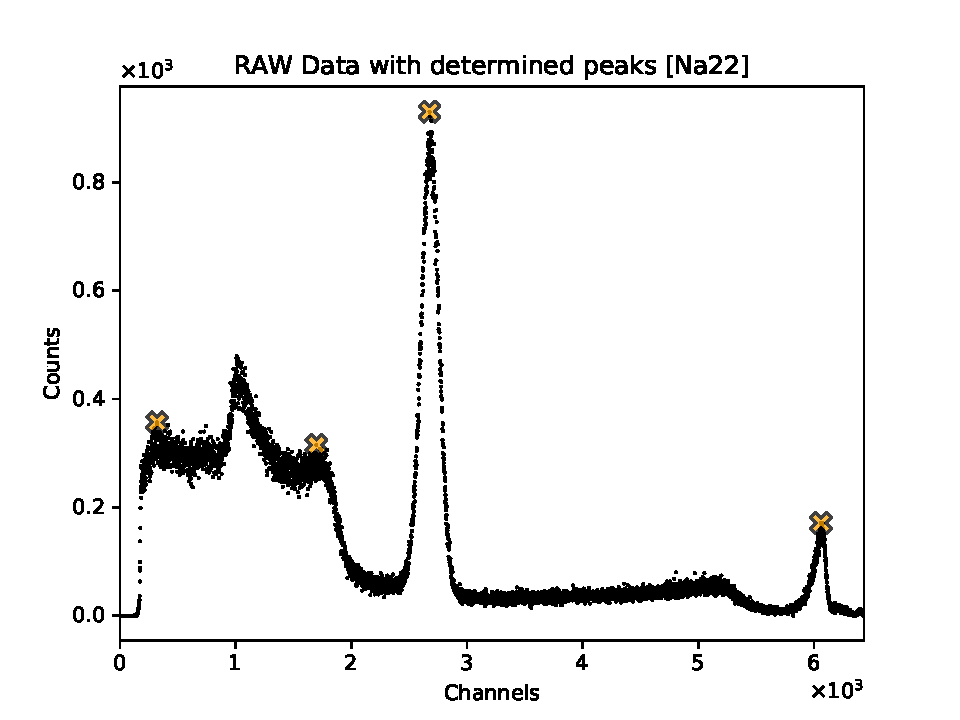
\includegraphics[width = .33\textwidth,trim={.1cm 0 1cm 0}, clip]{Immagini/RawNa22_with_determined_peaks.pdf}}\\
	\subfloat{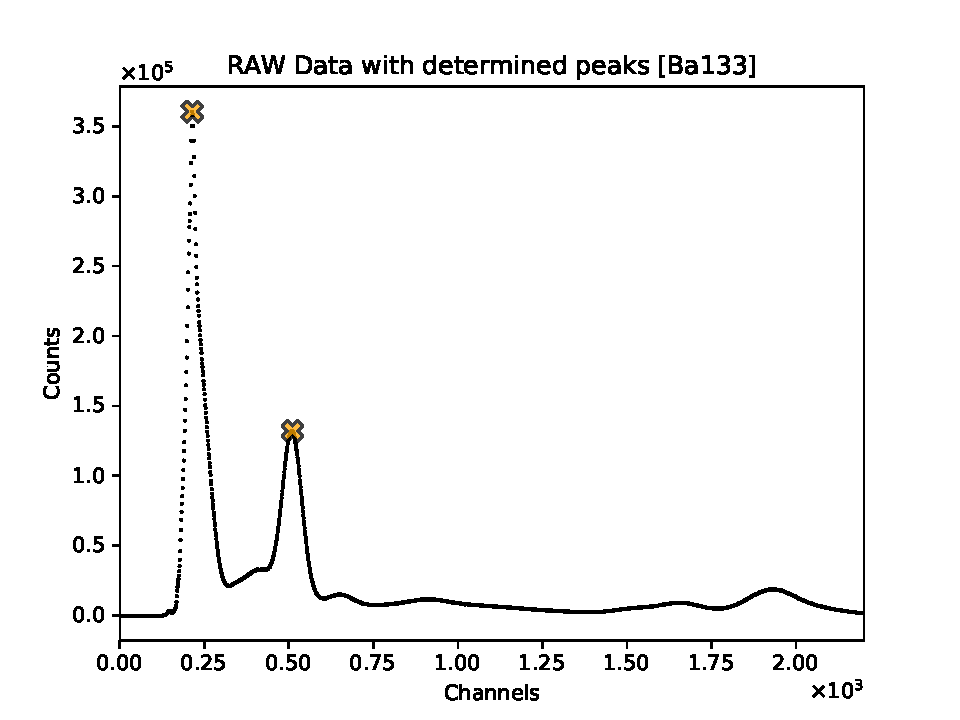
\includegraphics[width = .33\textwidth,trim={.1cm 0 1cm 0}, clip]{Immagini/RawBa133_with_determined_peaks.pdf}}
	\subfloat{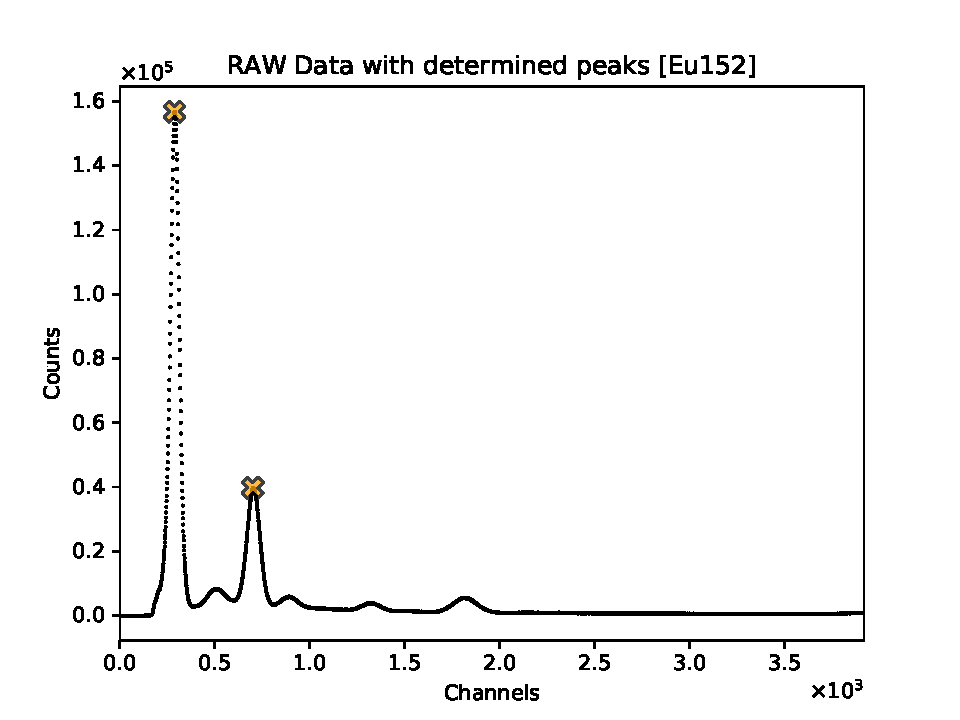
\includegraphics[width = .33\textwidth,trim={.1cm 0 1cm 0}, clip]{Immagini/RawEu152_with_determined_peaks.pdf}}
	\label{fig:PeakSearchRaw}
\end{sidewaysfigure}

\newpage

\begin{lstlisting}[language=python, style=Pystyle, caption=\texttt{Python} code for Spectral Peak Recognition Routine, label=list:PeakRoutine, 	captionpos=t]
""" Standard Libraries """
import numpy as np
import pylab as plt
from math import *

""" I/O Libraries """
import os
import sys

""" Best-Fit Library """
from scipy.optimize import curve_fit

########################################################################################

## Choosing the source

SourceName = str(input('Insert the desired source [Cs137|Co57|Na22|Ba133|Eu152]: '))

## Opening the ASCII file related to the chosen source

def get_script_path():
	return os.path.dirname(os.path.realpath(sys.argv[0]))

path = get_script_path()
data=np.loadtxt(path+'/Script&Data/CeBr3_'+SourceName+'.dat')

## Defining Effective-Range

i = len(data)
while(data[i-1] <= 0.01*np.max(data)/2): 
i = i - 1

x_max = i
data = data[range(1,x_max)]

## Plotting retrieved experimental data

x = np.array(range(1,x_max))
y = data

plt.figure('Raw'+SourceName)
plt.plot(x,y,'ko',markersize=0.5)
plt.xlim((1, x_max))
plt.xlabel('Channels')
bottom, top = plt.ylim()
plt.ylabel('Counts')
plt.title('RAW Data ['+SourceName+']')
plt.ticklabel_format(axis='both',style='sci',scilimits=(0,0),useMathText=True)
plt.show()

##############################
## Peak-Recognition Routine ##
##############################

# Derivatives of data
y1 = np.gradient(y)
y2 = np.gradient(y1)

X_Peaks1 = np.array([])
Y_Peaks1 = np.array([])
X_Peaks2 = np.array([])
Y_Peaks2 = np.array([])
Y1 = np.array([])
Y2 = np.array([])

steps = 20
for i in range(1,steps+1):
	
	# Minimization only in a partial domain
	X = x[(x > (x_max/steps)*(i-1)) & (x <= (x_max/steps)*i)]
	Y = y[(x > (x_max/steps)*(i-1)) & (x <= (x_max/steps)*i)]
	Y1 = y1[(x > (x_max/steps)*(i-1)) & (x <= (x_max/steps)*i)]
	Y2 = y2[(x > (x_max/steps)*(i-1)) & (x <= (x_max/steps)*i)]
	X_CandidatePeak = X[np.argmax(Y)]
	Y_CandidatePeak = np.max(Y)
	Y1_CandidatePeak = Y1[np.argmax(Y)]
	Y2_CandidatePeak = Y2[np.argmax(Y)]
	
	a = 1.1*np.max(Y)/2         # Threshold on Background
	b = 0.9*np.max(abs(Y1))/2   # Threshold on Slope
	c = 0.1*np.max(abs(Y2))/2   # Threshold on Concavity
	
	if (Y_CandidatePeak > a)and(abs(Y1_CandidatePeak)< b)and(Y2_CandidatePeak<-c)and(Y_CandidatePeak > 0.13*np.max(y)):
	
		X_Peaks1 = np.append(X_Peaks1, X_CandidatePeak)
		Y_Peaks1 = np.append(Y_Peaks1, Y_CandidatePeak)
	
steps = 8
for i in range(1,steps+1):
	
	# Minimization only in a partial domain
	X = x[(x > (x_max/steps)*(i-1)) & (x <= (x_max/steps)*i)]
	Y = y[(x > (x_max/steps)*(i-1)) & (x <= (x_max/steps)*i)]
	Y1 = y1[(x > (x_max/steps)*(i-1)) & (x <= (x_max/steps)*i)]
	Y2 = y2[(x > (x_max/steps)*(i-1)) & (x <= (x_max/steps)*i)]
	X_CandidatePeak = X[np.argmax(Y)]
	Y_CandidatePeak = np.max(Y)
	Y1_CandidatePeak = Y1[np.argmax(Y)]
	Y2_CandidatePeak = Y2[np.argmax(Y)]
	
	a = 1.1*np.max(Y)/2         # Threshold on Background
	b = 0.9*np.max(abs(Y1))/2   # Threshold on Slope
	c = 0.1*np.max(abs(Y2))/2   # Threshold on Concavity
	
	if (Y_CandidatePeak > a)and(abs(Y1_CandidatePeak)< b)and(Y2_CandidatePeak<-c)and(Y_CandidatePeak > 0.13*np.max(y)):
	
		for j in range(len(X_Peaks1)):
			if X_CandidatePeak == X_Peaks1[j]:
				X_Peaks2 = np.append(X_Peaks2, X_CandidatePeak)
				Y_Peaks2 = np.append(Y_Peaks2, Y_CandidatePeak)

# Showing determined peaks
plt.figure('Raw'+SourceName+' with determined peaks')
plt.plot(x,y,'ko',markersize=0.5)
plt.xlim((1, x_max))
plt.xlabel('Channels')
bottom, top = plt.ylim()
plt.ylabel('Counts')
plt.title('RAW Data with determined peaks ['+SourceName+']')
plt.ticklabel_format(axis='both',style='sci',scilimits=(0,0),useMathText=True)
plt.show()
plt.plot(X_Peaks2,Y_Peaks2,'X',c='orange',markeredgecolor='k',markersize=10,alpha=0.75)

## Principal-Peak [P.P] Analysis

xmax_peak = X_Peaks2[np.argmax(Y_Peaks2)]   # Principal-Peak position
ymax_peak = np.max(Y_Peaks2)                # Principal-Peak value
index = np.where(x==xmax_peak)[0]           # Finding P.P in our data array

########################################################################################
# Definition of a ROI: we must have |yROI-yPeak|<=d and |yROI'|<t, on both sides of P.P.
########################################################################################
d = ymax_peak*0.75 # -----------------------
t = 50             # BEST VALUES [HEURISTIC]
#################### -----------------------

x1=x[(abs(y1)<t) & (x<xmax_peak) & (abs(y-ymax_peak)>d)]
index1=np.where(x==x1[abs(x1-xmax_peak)==min(abs(x1-xmax_peak))])[0]
i1=np.array(index1[0])
x2=x[(abs(y1)<t) & (x>xmax_peak) & (abs(y-ymax_peak)>d)]
index2=np.where(x==x2[abs(x2-xmax_peak)==min(abs(x2-xmax_peak))])[0]
i2=np.array(index2[0])
xnew=x[i1:i2]
ynew=y[i1:i2]

#Plotting the ROI-confined Peak
plt.figure('Peak-Fitting_'+SourceName)
plt.plot(x[range(i1-1,i2+1)],y[range(i1-1,i2+1)],'ko',markersize=1.5,label='ROI-data')

# Background Esimate: Linear-Fit beetwen ROI edges... 
a=xnew[0]
b=xnew[len(xnew)-1]
x_to_fit = np.array([xnew[0],xnew[len(xnew)-1]])
y_to_fit = np.array([ynew[0],ynew[len(xnew)-1]])
coefficients = np.polyfit(x_to_fit, y_to_fit, deg=1) # Linear-Fit
polynomial = np.poly1d(coefficients)                 # ----------
x_pol = np.linspace(xnew[0],xnew[len(xnew)-1],100)
y_pol = polynomial(x_pol)
plt.plot(x_pol,y_pol,'m-.',linewidth=1.5,alpha=0.5,label='Background')

# Background-correcting the Peak [and plotting]
ynew=ynew-polynomial(xnew)
plt.plot(xnew,ynew,'o',c='orange',markersize=1.5,label='Corrected-Peak')
plt.ylim(0,ymax_peak*2-1.25*d)

## Gaussian Best-Fit of the corrected P.P. data

def Gauss(x,A,x0,sigma):
return A*np.exp(-(x-x0)**2/(2*sigma**2))

A_init = np.max(ynew)       # -----------
x0_init = np.mean(xnew)     # First guess
sigma_init = np.std(xnew)   # -----------

# Least-Squares Fitting...
popt,pcov = curve_fit(Gauss,xnew,ynew,p0=[A_init,x0_init,sigma_init])

A = popt[0]                                  # ----------------
x0 = popt[1]                                 # Best-Fit results
sigma = popt[2]                              # ----------------
StDev_vec = 2.3548200*np.sqrt(np.diag(pcov)) # ----------------

W = 2.3548200*popt[2] # Peak-Width: FWHM
S = 0.5*A*W # Area with Triangle-Approx.
R = W/x0 # Resolution: FWHM/x0

dA = StDev_vec[0]
dx = StDev_vec[1]
dW = 2.3548200*StDev_vec[2]
dS = (dA/A + dW/W)*S
dR = (dW/W + dx/x0)*R

# Printing Results...
print('PRINCIPAL-PEAK POSITION', x0,''"$\pm$", dx)
print('PRINCIPAL-PEAK HEIGHT: ', A,''"$\pm$", dA)
print('PRINCIPAL-PEAK WIDTH: ', W,''"$\pm$", dW)
print('PRINCIPAL-PEAK AREA :', S,''"$\pm$", dS)
print('CRYSTAL RESOLUTION: ', R,''"$\pm$", dR)

# Plotting & Showing All
yFIT = Gauss(xnew,A,x0,sigma)
plt.plot(xnew,yFIT,'g--',linewidth=1.5,label='Gaussian-Fit')
plt.title('Principal Peak Best-Fitting ['+SourceName+']')
plt.ticklabel_format(axis='both',style='sci',scilimits=(0,0),useMathText=True)
plt.legend(markerscale=3)
plt.show()
\end{lstlisting}

\begin{figure}[h!]
	\centering
	\caption{Analisi su dati grezzi del Picco Principale (P.P.) della sorgente Cs$^{137}$. }
	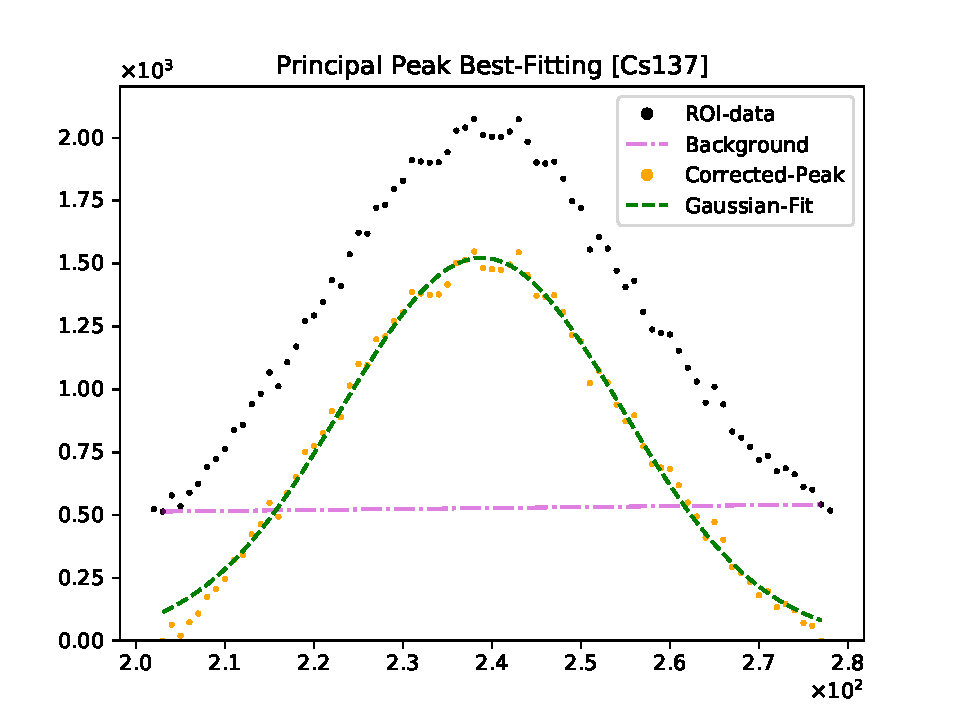
\includegraphics[width =  \textwidth,trim={1cm 0 1cm 0}, clip]{Immagini/Peak-Fitting_Cs137_RAW.pdf}
	\label{fig:PPRawCs137} \bigskip\bigskip
	\begin{lstlisting}[language=python, style=Pystyle, mathescape=true]
	>>> (executing file "PhytonCodeEs5.py")
	Insert the desired source [Cs137|Co57|Na22|Ba133|Eu152]: Cs137
	PRINCIPAL-PEAK POSITION 238.8467517967467 $\pm$ 0.3098839895739907
	PRINCIPAL-PEAK HEIGHT:  1523.3400945401845 $\pm$ 26.00320803587605
	PRINCIPAL-PEAK WIDTH:  37.09865495020793 $\pm$ 0.7485587193418013
	PRINCIPAL-PEAK AREA : 28256.934269581718 $\pm$ 1052.4967764062292
	CRYSTAL RESOLUTION:  0.15532409241963677 $\pm$ 0.003335574642671817
	\end{lstlisting} \bigskip\bigskip
\end{figure}

\newpage

\begin{figure}[h!]
	\centering
	\caption{Analisi su dati grezzi del Picco Principale (P.P.) della sorgente Co$^{57}$. }
	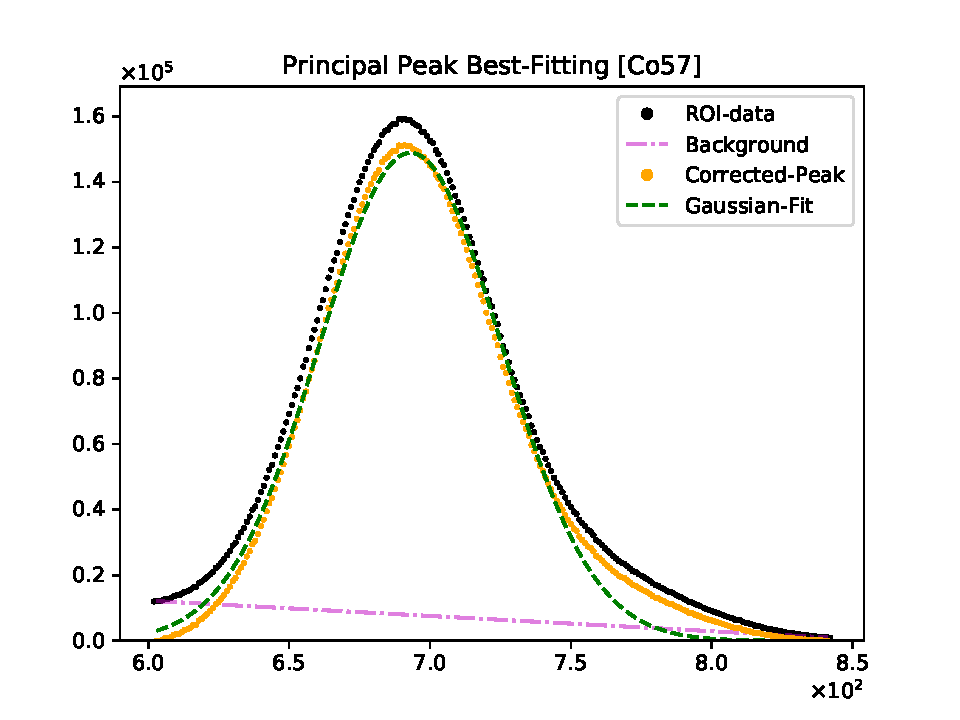
\includegraphics[width =  \textwidth,trim={1cm 0 1cm 0}, clip]{Immagini/Peak-Fitting_Co57_RAW.pdf}
	\label{fig:PPRawCo57} \bigskip\bigskip
	\begin{lstlisting}[language=python, style=Pystyle, mathescape=true]
	>>> (executing file "PhytonCodeEs5.py")
	Insert the desired source [Cs137|Co57|Na22|Ba133|Eu152]: Co57
	PRINCIPAL-PEAK POSITION 693.1137861569199 $\pm$ 0.4433360809406253
	PRINCIPAL-PEAK HEIGHT:  148880.4511121081 $\pm$ 1769.474256713379
	PRINCIPAL-PEAK WIDTH:  76.09652174560256 $\pm$ 1.04632416144232
	PRINCIPAL-PEAK AREA : 5664642.242773826 $\pm$ 145214.0247096522
	CRYSTAL RESOLUTION:  0.10978936397663056 $\pm$ 0.0015798239331929512
	\end{lstlisting} \bigskip\bigskip
\end{figure}

\newpage

\begin{figure}[h!]
	\centering
	\caption{Analisi su dati grezzi del Picco Principale (P.P.) della sorgente Na$^{22}$. }
	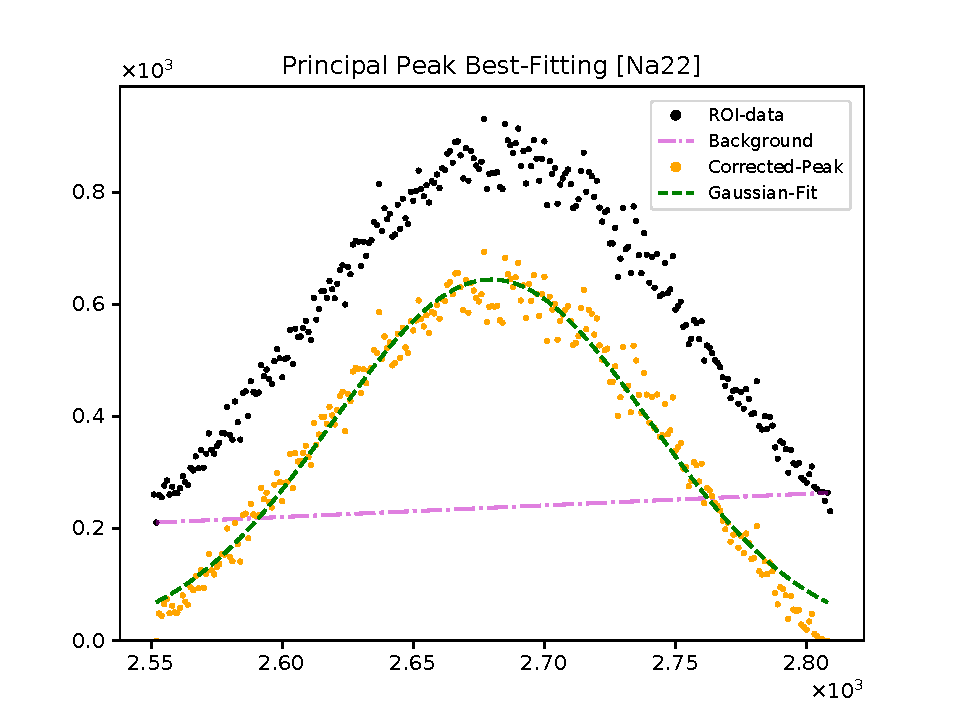
\includegraphics[width =  \textwidth,trim={1cm 0 1cm 0}, clip]{Immagini/Peak-Fitting_Na22_RAW.pdf}
	\label{fig:PPRawNa22} \bigskip\bigskip
	\begin{lstlisting}[language=python, style=Pystyle, mathescape=true]
	>>> (executing file "PhytonCodeEs5.py")
	Insert the desired source [Cs137|Co57|Na22|Ba133|Eu152]: Na22
	PRINCIPAL-PEAK POSITION 2679.8233949851183 $\pm$ 1.0636289671764676
	PRINCIPAL-PEAK HEIGHT:  644.6055128147791 $\pm$ 9.837826754288718
	PRINCIPAL-PEAK WIDTH:  142.39273009203848 $\pm$ 2.6530917116409816
	PRINCIPAL-PEAK AREA : 45893.56940103744 $\pm$ 1555.5162765213215
	CRYSTAL RESOLUTION:  0.05313511717171542 $\pm$ 0.0010111143019759258
	\end{lstlisting} \bigskip\bigskip
\end{figure}

\newpage

\begin{figure}[h!]
	\centering
	\caption{Analisi su dati grezzi del Picco Principale (P.P.) della sorgente Ba$^{133}$. }
	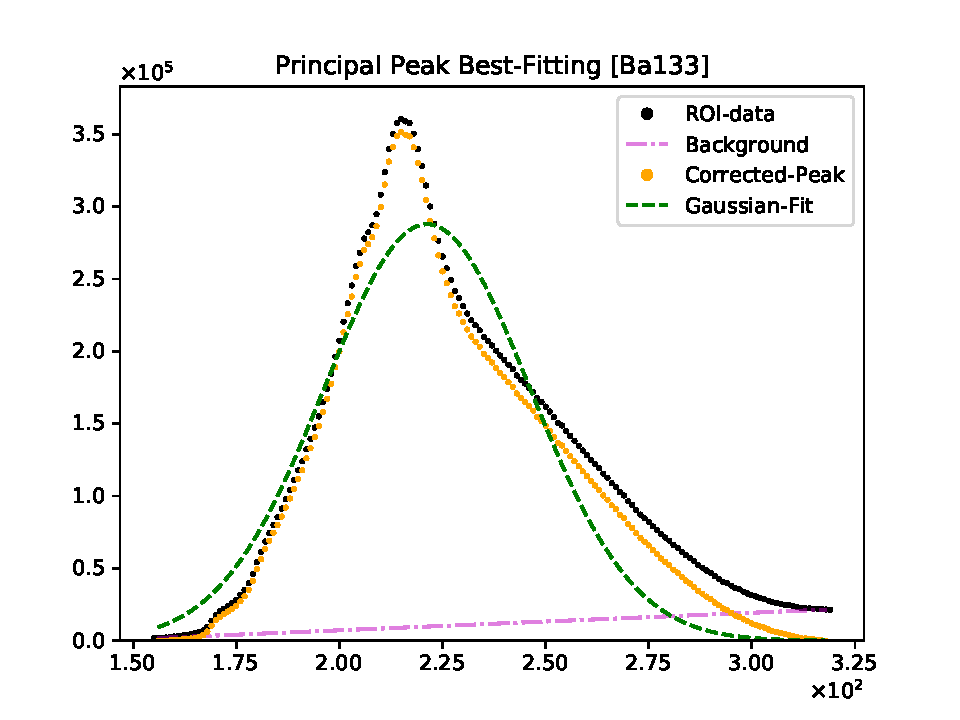
\includegraphics[width =  \textwidth,trim={1cm 0 1cm 0}, clip]{Immagini/Peak-Fitting_Ba133_RAW.pdf}
	\label{fig:PPRawBa133} \bigskip\bigskip
	\begin{lstlisting}[language=python, style=Pystyle, mathescape=true]
	>>> (executing file "PhytonCodeEs5.py")
	Insert the desired source [Cs137|Co57|Na22|Ba133|Eu152]: Ba133
	PRINCIPAL-PEAK POSITION 221.25212247553907 $\pm$ 1.2732933530258672
	PRINCIPAL-PEAK HEIGHT:  287864.93020777084 $\pm$ 12741.050893987342
	PRINCIPAL-PEAK WIDTH:  58.70101313148694 $\pm$ 3.0122036998891812
	PRINCIPAL-PEAK AREA : 8448981.524110464 $\pm$ 807510.2018385414
	CRYSTAL RESOLUTION:  0.2653127684141278 $\pm$ 0.01514120925440681
	\end{lstlisting} \bigskip\bigskip
\end{figure}

\newpage

\begin{figure}[h!]
	\centering
	\caption{Analisi su dati grezzi del Picco Principale (P.P.) della sorgente Eu$^{152}$. }
	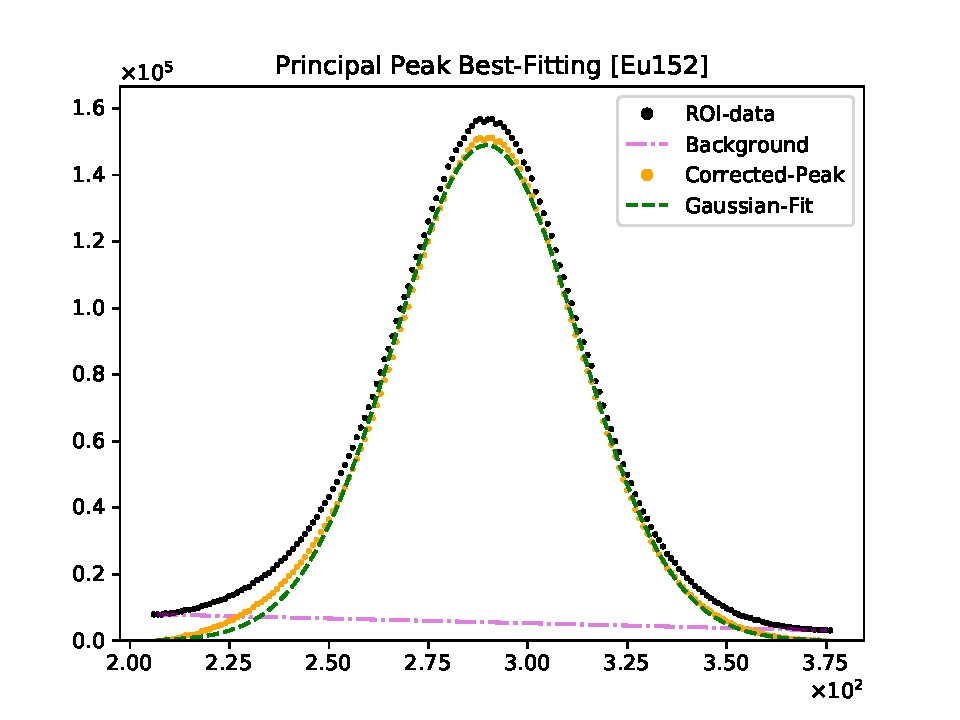
\includegraphics[width =  \textwidth,trim={1cm 0 1cm 0}, clip]{Immagini/Peak-Fitting_Eu152_RAW.pdf}
	\label{fig:PPRawEu152} \bigskip\bigskip
	\begin{lstlisting}[language=python, style=Pystyle, mathescape=true]
	>>> (executing file "PhytonCodeEs5.py")
	Insert the desired source [Cs137|Co57|Na22|Ba133|Eu152]: Eu152
	PRINCIPAL-PEAK POSITION 289.67056608195855 $\pm$ 0.15968983090396094
	PRINCIPAL-PEAK HEIGHT:  149000.1993161386 $\pm$ 887.0254434869172
	PRINCIPAL-PEAK WIDTH:  54.704433482585735 $\pm$ 0.3760595236985809
	PRINCIPAL-PEAK AREA : 4075485.7461908604 $\pm$ 52278.58417820594
	CRYSTAL RESOLUTION:  0.18885050774232898 $\pm$ 0.0014023414074840683
	\end{lstlisting} \bigskip\bigskip
\end{figure}

\newpage

\noindent Complessivamente l'analisi operata sui dati grezzi risulta ragionevole: i valori di incertezza sui parametri di \emph{best-fit} sono almeno di due ordini di grandezza inferiori al relativo valore stimato in tutti casi meno che per il P.P del Ba$^{133}$, che ha profilo palesemente non gaussiano. Osserviamo che la risoluzione spettrale dei picchi risulta migliore per le risonanze a energie inferiori, per cui deduciamo che il cristallo abbia risoluzione decrescente con l'energia di eccitazione: di ciò abbiamo trovato riscontro in letteratura\footnote{\href{http://www.sympnp.org/proceedings/62/G51.pdf}{G. Mishra \emph{et al.}, Proc. \!DAE Symp. \!\!Nucl. \!\!Phys. \!\!62 (2017) 1092-1093\\ \href{https://doi.org/10.1016/j.nima.2013.08.005}{F. Quarati \emph{et al.}, Nuclear Instruments and Methods in Physics Research A 729 (2013) 596–604}}}. Per quanto riguarda le proprietà di risposta del cristallo abbiamo invece confrontato direttamente gli istogrammi grezzi in \figurename~\ref{fig:RAW} con gli spettri di emissione riportati su \href{https://www.gammaspectacular.com}{\texttt{Gamma \!\!Spectacular}} per alcune delle sorgenti considerate\footnote{In particolare per Na$^{22}$ e Ba$^{133}$ riconoscendone i picchi rispettivamente a 511~keV e 1274~kev e a 31~keV e 81~keV.} e dedotto che il cristallo non presenta una buona linearità se non nel limite di alte energie.

\[* * * \] \smallskip

\noindent Per operare lo {smoothing} dei dati si è adoperata la libreria \texttt{scipy.ndimage.gaussian\_filter}\footnote{Documentazione: \href{https://docs.scipy.org/doc/scipy/reference/generated/scipy.ndimage.gaussian_filter.html}{\texttt{https://docs.scipy.org/doc/scipy/reference/generated/scipy.ndimage.gaussian\_filter.html}}} di \texttt{Python}, ottenendo i risultati riportati in \figurename~\ref{fig:Smoothing} secondo il codice di seguito riportato:

\vfill

\begin{lstlisting}[language=python, style=Pystyle, caption=\texttt{Python} code for Gaussian Smoothing Routine, label=list:Smoothing, 	captionpos=b]
""" Gaussian-Smoothing Library """
from scipy.ndimage import gaussian_filter as smoothing

## Smoothing Data
y=smoothing(data,sigma=5)

## Plotting Results
plt.figure('Smoothing'+SourceName)
plt.plot(x,data,'ko',markersize=0.5,label='RAW Data')
plt.plot(x,y,'ro',markersize=0.5,label='Smoothed')
plt.xlim((1, x_max))
plt.xlabel('Channels')
plt.ylim((bottom, top))
plt.ylabel('Counts')
plt.title('Smoothing ['+SourceName+']')
plt.legend(markerscale=10)
plt.ticklabel_format(axis='both',style='sci',scilimits=(0,0),useMathText=True)
plt.figure('Smoothed'+SourceName)
plt.plot(x,y,'ro',markersize=0.5)
plt.xlim((1, x_max))
plt.xlabel('Channels')
plt.ylim((bottom, top))
plt.ylabel('Counts')
plt.title('Smoothed Data with determined peaks ['+SourceName+']')
plt.ticklabel_format(axis='both',style='sci',scilimits=(0,0),useMathText=True)
plt.show()
\end{lstlisting}

\vfill

\noindent L'applicazione della medesima routine (Listato~\ref{list:PeakRoutine} a partire dalla riga 50) sui dati sottoposti a smoothing porta a individuare i picchi riportati in \figurename~\ref{fig:PeakSearchSmoothed}, in cui possiamo osservare come le risonanze trascurate in precedenza su Co$^{57}$ e Na$^{22}$ vengano adesso correttamente riconosciute. Infine osserviamo che l'analisi del P.P. risulta notevolmente migliorata dal processo di smoothing, con un generale miglioramento delle incertezze associate ai parametri del modello Gaussiano. Tuttavia possiamo notare come l'altezza dei picchi si riduca sistematicamente passando dai dati grezzi a quelli sottoposti a smoothing e viceversa cresca la larghezza dei picchi: ne deduciamo che lo smoothing, pur aiutando nella determinazione e analisi dei picchi, introduce dei bias sulla stima di alcuni parametri fisici, quali ad esempio la risoluzione spettrale del cristallo.

\vfill

\begin{sidewaysfigure}
	\centering
	\caption{Smoothing dei cinque spettri di calibrazione considerati.}
	\subfloat{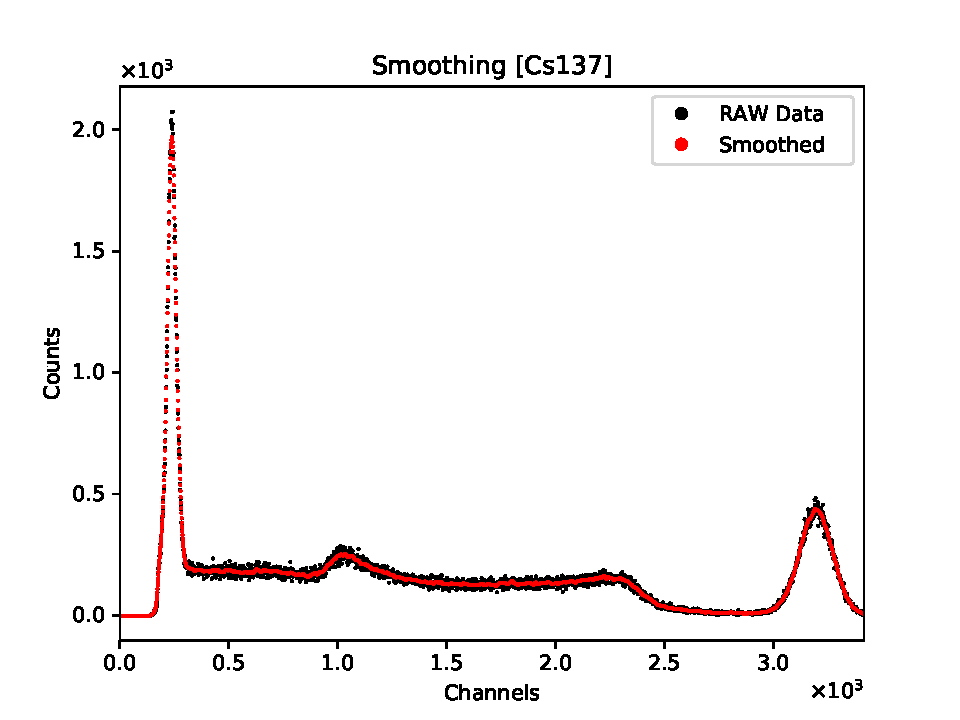
\includegraphics[width = .33\textwidth,trim={.1cm 0 1cm 0}, clip]{Immagini/SmoothingCs137.pdf}} 
	\subfloat{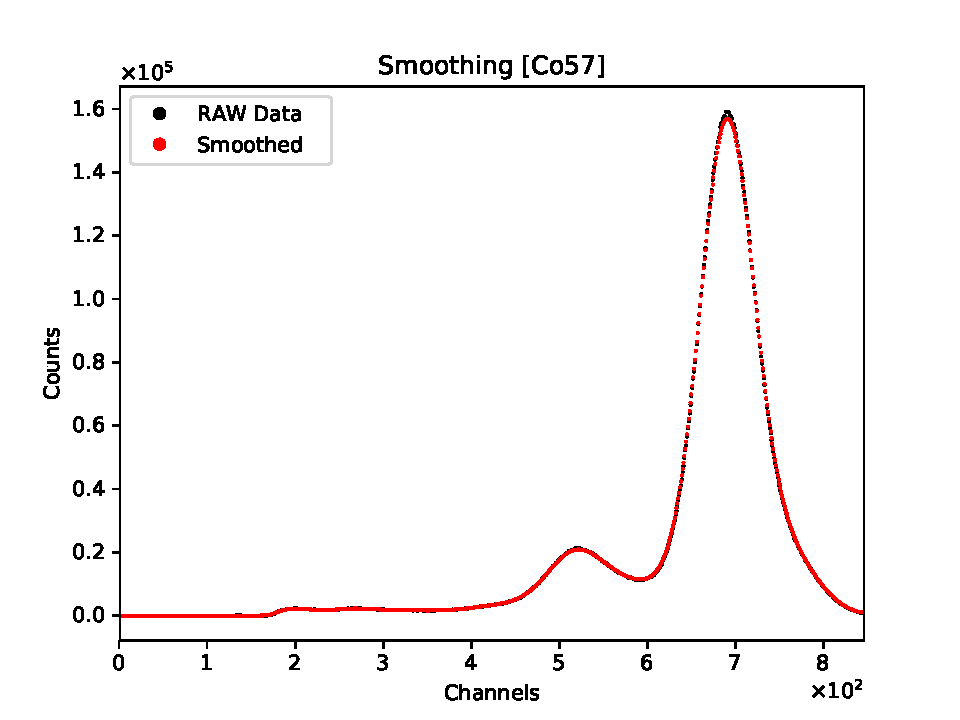
\includegraphics[width =  .33\textwidth,trim={.1cm 0 1cm 0}, clip]{Immagini/SmoothingCo57.pdf}}
	\subfloat{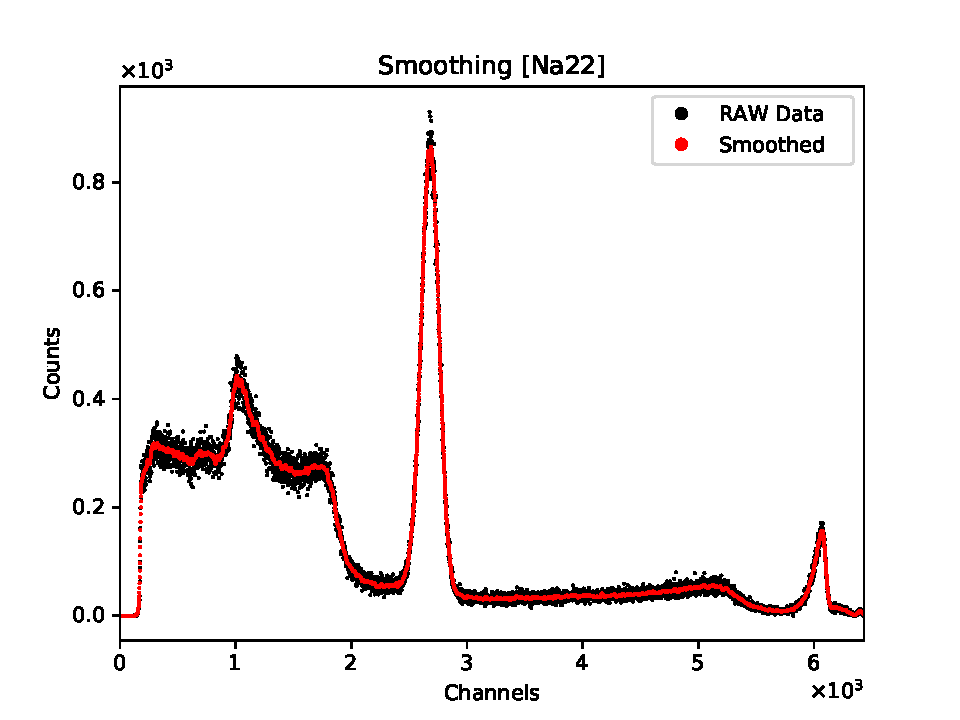
\includegraphics[width = .33\textwidth,trim={.1cm 0 1cm 0}, clip]{Immagini/SmoothingNa22.pdf}}\\
	\subfloat{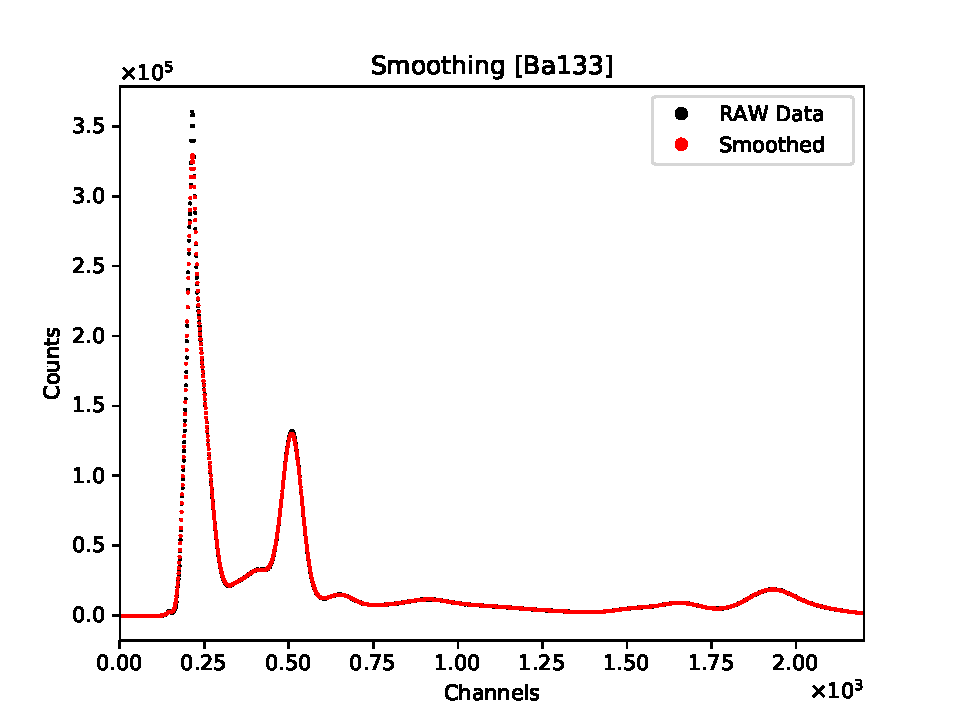
\includegraphics[width = .33\textwidth,trim={.1cm 0 1cm 0}, clip]{Immagini/SmoothingBa133.pdf}}
	\subfloat{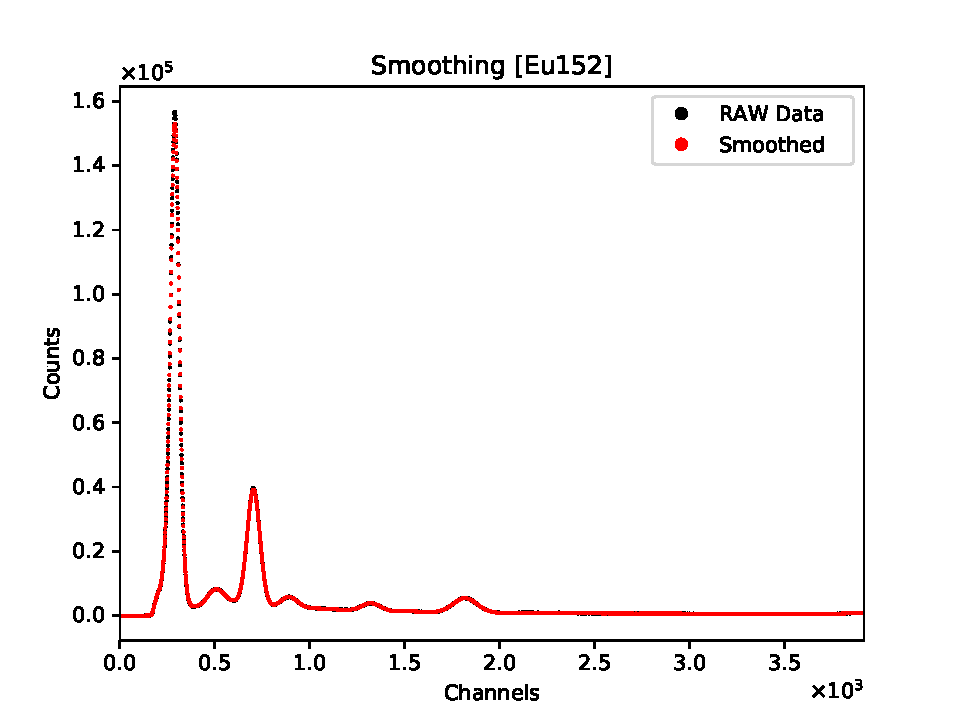
\includegraphics[width = .33\textwidth,trim={.1cm 0 1cm 0}, clip]{Immagini/SmoothingEu152.pdf}}
	\label{fig:Smoothing}
\end{sidewaysfigure}

\begin{sidewaysfigure}
	\centering
	\caption{Ricerca dei picchi di scintillazione sugli spettri di calibrazione sottoposti a {smoothing}.}
	\subfloat{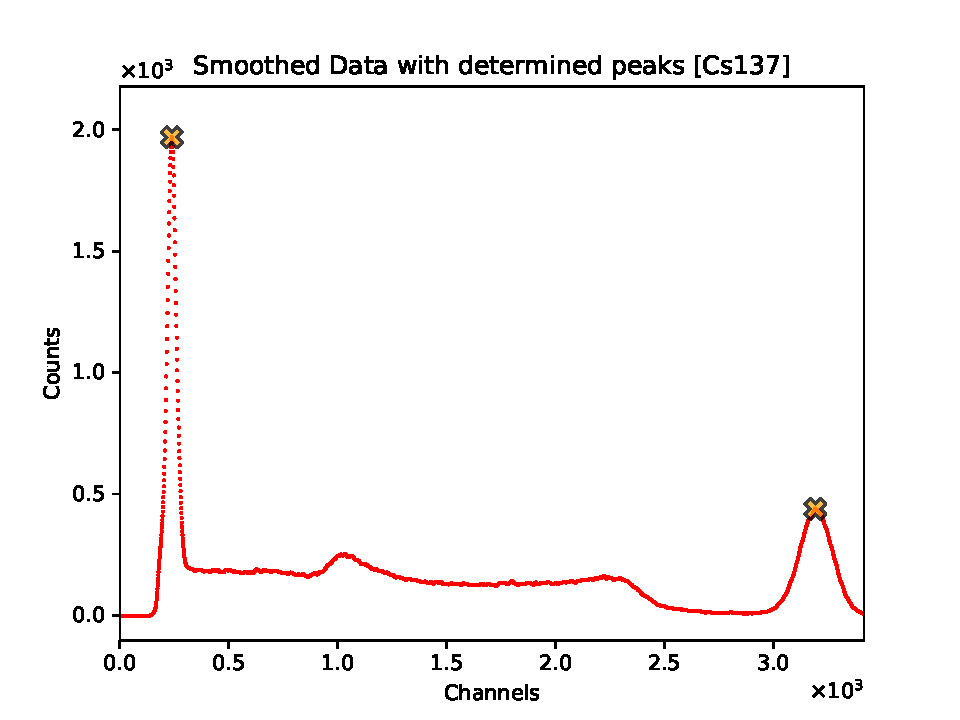
\includegraphics[width = .33\textwidth,trim={.1cm 0 1cm 0}, clip]{Immagini/SmoothedCs137.pdf}} 
	\subfloat{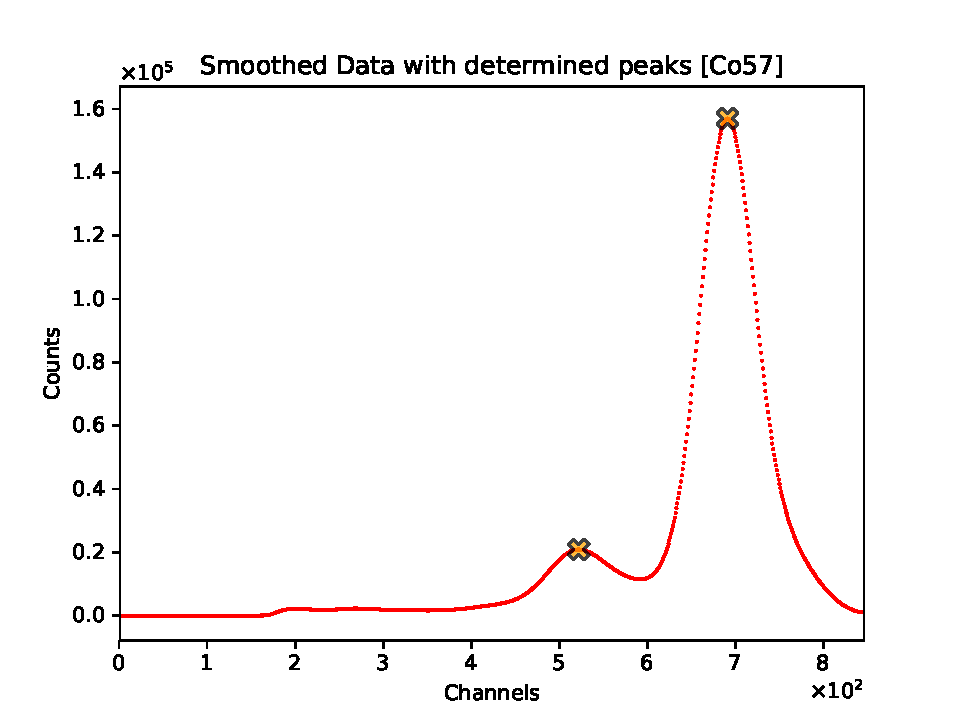
\includegraphics[width =  .33\textwidth,trim={.1cm 0 1cm 0}, clip]{Immagini/SmoothedCo57.pdf}}
	\subfloat{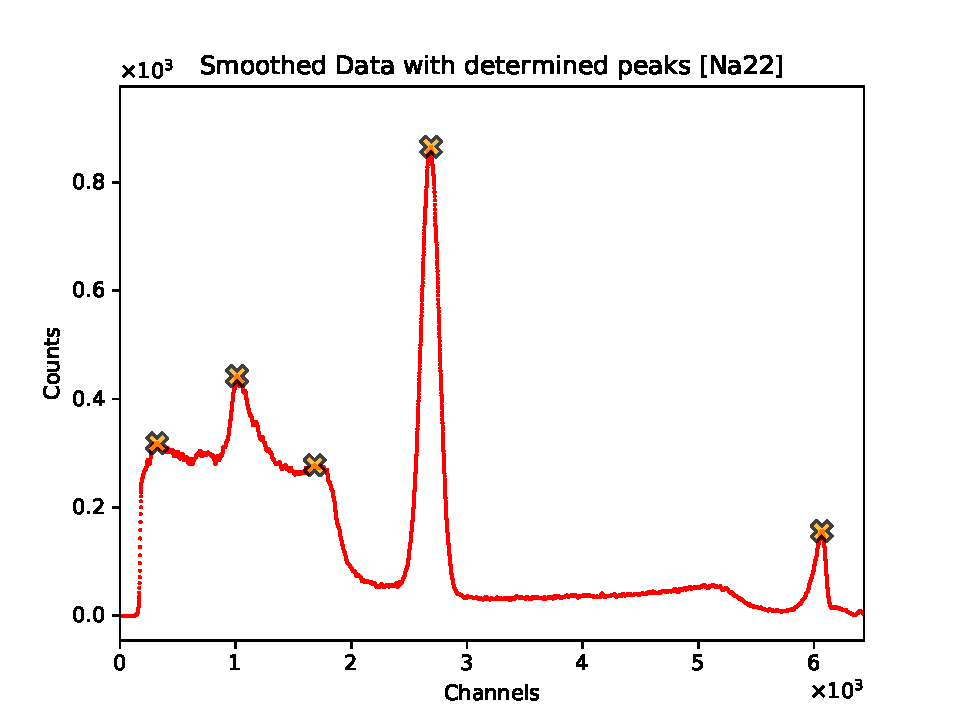
\includegraphics[width = .33\textwidth,trim={.1cm 0 1cm 0}, clip]{Immagini/SmoothedNa22.pdf}}\\
	\subfloat{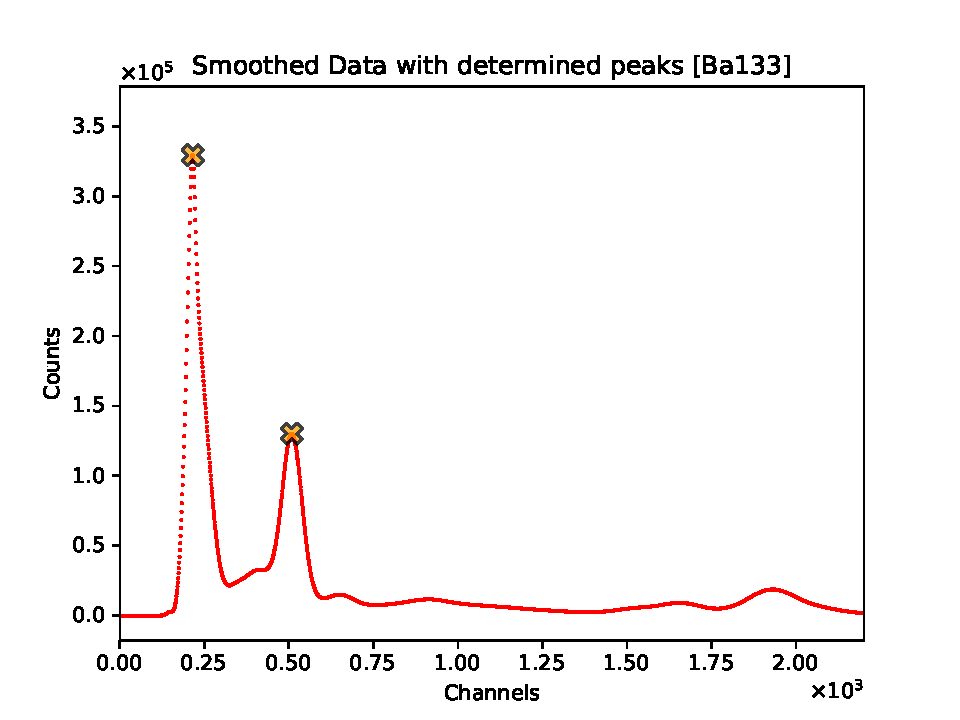
\includegraphics[width = .33\textwidth,trim={.1cm 0 1cm 0}, clip]{Immagini/SmoothedBa133.pdf}}
	\subfloat{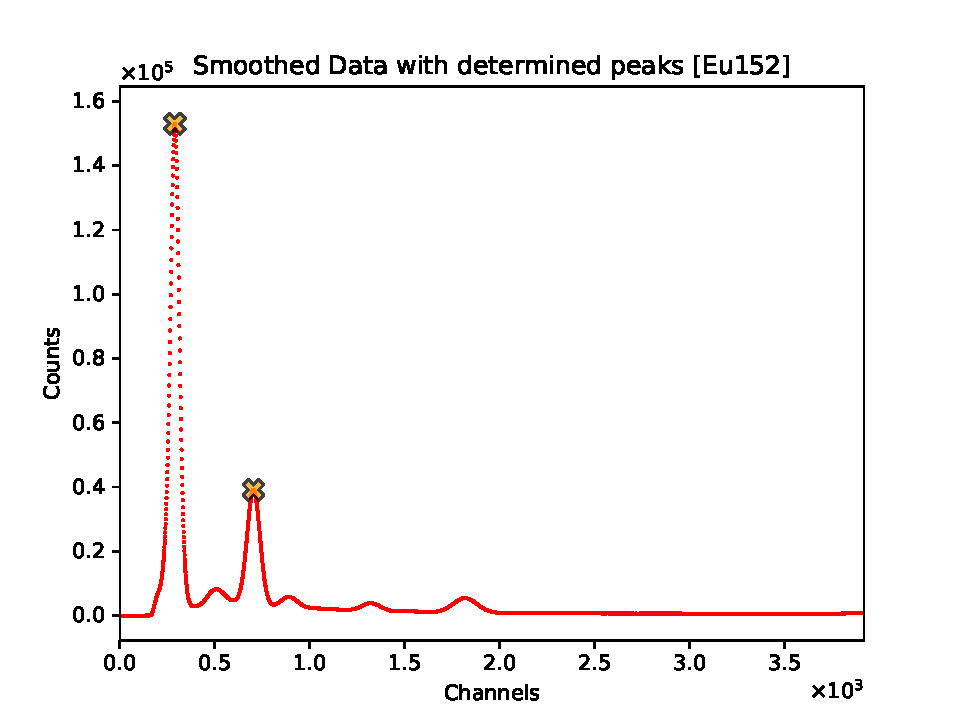
\includegraphics[width = .33\textwidth,trim={.1cm 0 1cm 0}, clip]{Immagini/SmoothedEu152.pdf}}
	\label{fig:PeakSearchSmoothed}
\end{sidewaysfigure}

\begin{figure}[h!]
	\centering
	\caption{Analisi su dati \emph{smoothed} del Picco Principale (P.P.) della sorgente Cs$^{137}$. }
	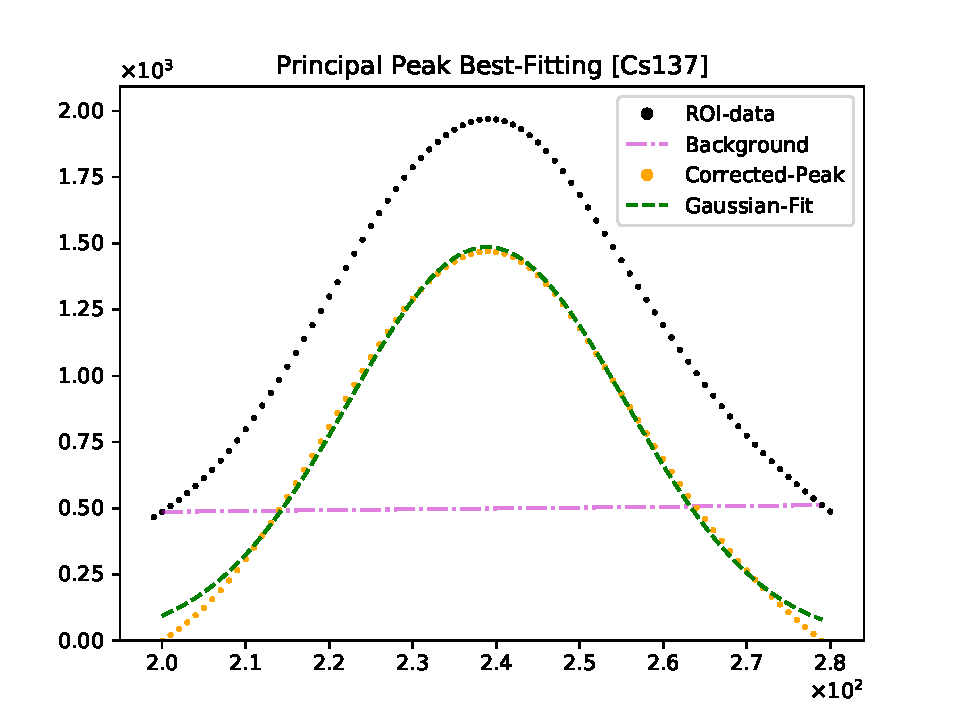
\includegraphics[width =  \textwidth,trim={1cm 0 1cm 0}, clip]{Immagini/Peak-Fitting_Cs137.pdf}
	\label{fig:PPCs137} \bigskip\bigskip
	\begin{lstlisting}[language=python, style=Pystyle, mathescape=true]
	>>> (executing file "PhytonCodeEs5.py")
	Insert the desired source [Cs137|Co57|Na22|Ba133|Eu152]: Cs137
	PRINCIPAL-PEAK POSITION 238.91761912451213 $\pm$ 0.22132312943379565
	PRINCIPAL-PEAK HEIGHT:  1486.306984085268 $\pm$ 17.214673725913784
	PRINCIPAL-PEAK WIDTH:  39.04930494268223 $\pm$ 0.5329330173241219
	PRINCIPAL-PEAK AREA : 29019.62732999198 $\pm$ 732.1615547552321
	CRYSTAL RESOLUTION:  0.16344255013830372 $\pm$ 0.0023820203637086343
	\end{lstlisting}\bigskip\bigskip
\end{figure}

\newpage

\begin{figure}[h!]
	\centering
	\caption{Analisi su dati \emph{smoothed} del Picco Principale (P.P.) della sorgente Co$^{57}$. }
	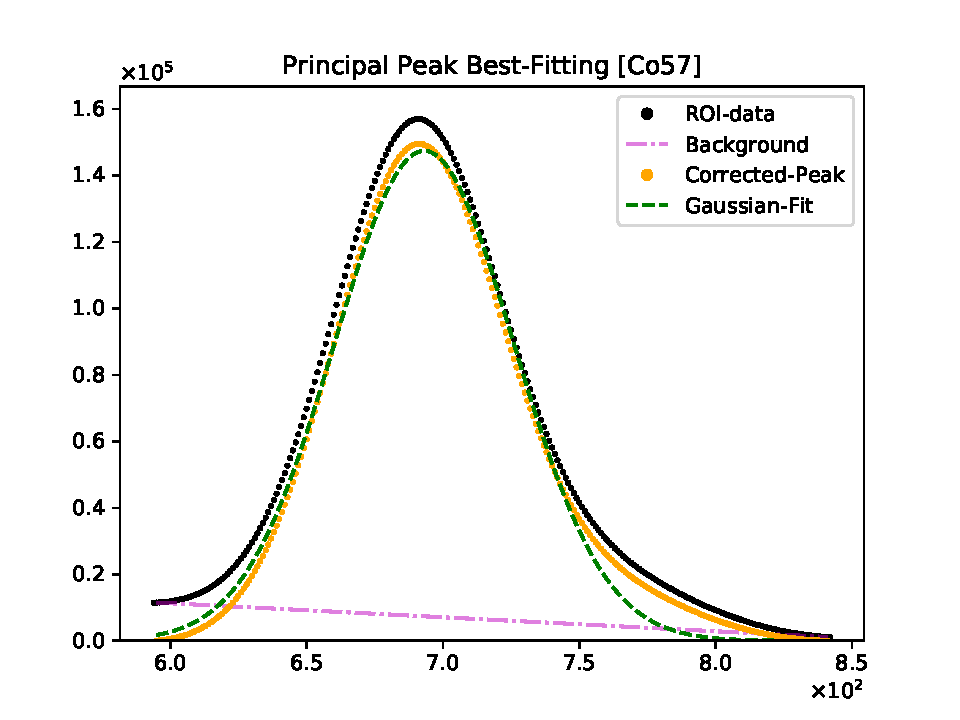
\includegraphics[width =  \textwidth,trim={1cm 0 1cm 0}, clip]{Immagini/Peak-Fitting_Co57.pdf}
	\label{fig:PPCo57} \bigskip\bigskip
	\begin{lstlisting}[language=python, style=Pystyle, mathescape=true]
	>>> (executing file "PhytonCodeEs5.py")
	Insert the desired source [Cs137|Co57|Na22|Ba133|Eu152]: Co57
	PRINCIPAL-PEAK POSITION 693.1196439613678 $\pm$ 0.42736955821149747
	PRINCIPAL-PEAK HEIGHT:  147417.44636429526 $\pm$ 1658.6905056705684
	PRINCIPAL-PEAK WIDTH:  77.4723612953905 $\pm$ 1.007283111318557
	PRINCIPAL-PEAK AREA : 5710388.832989266 $\pm$ 138496.887084504
	CRYSTAL RESOLUTION:  0.11177343186035649 $\pm$ 0.0015221782887043748
	\end{lstlisting}\bigskip\bigskip
\end{figure}

\newpage

\begin{figure}[h!]
	\centering
	\caption{Analisi su dati \emph{smoothed} del Picco Principale (P.P.) della sorgente Na$^{22}$. }
	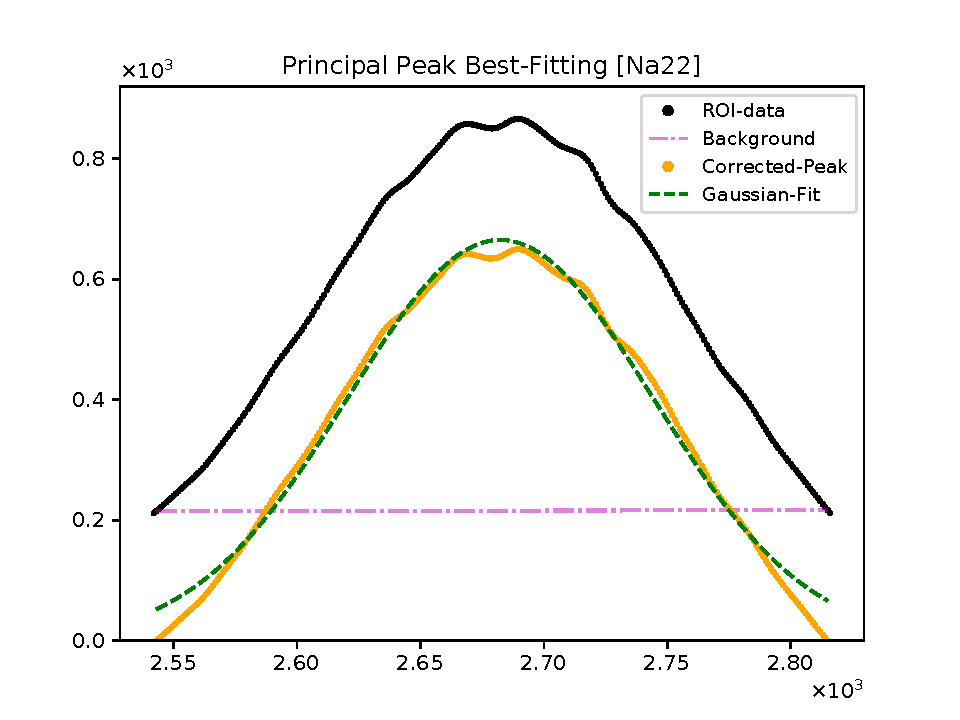
\includegraphics[width =  \textwidth,trim={1cm 0 1cm 0}, clip]{Immagini/Peak-Fitting_Na22.pdf}
	\label{fig:PPNa22} \bigskip\bigskip
	\begin{lstlisting}[language=python, style=Pystyle, mathescape=true]
	>>> (executing file "PhytonCodeEs5.py")
	Insert the desired source [Cs137|Co57|Na22|Ba133|Eu152]: Na22
	PRINCIPAL-PEAK POSITION 2682.367779401036 $\pm$ 0.6482369680134931
	PRINCIPAL-PEAK HEIGHT:  665.286115220424 $\pm$ 6.054778595618799
	PRINCIPAL-PEAK WIDTH:  145.5665828324627 $\pm$ 1.596600338802527
	PRINCIPAL-PEAK AREA : 48421.71319926059 $\pm$ 971.7847334664561
	CRYSTAL RESOLUTION:  0.054267943400724585 $\pm$ 0.0006083352321870312
	\end{lstlisting}\bigskip\bigskip
\end{figure}

\newpage

\begin{figure}[h!]
	\centering
	\caption{Analisi su dati \emph{smoothed} del Picco Principale (P.P.) della sorgente Ba$^{133}$. }
	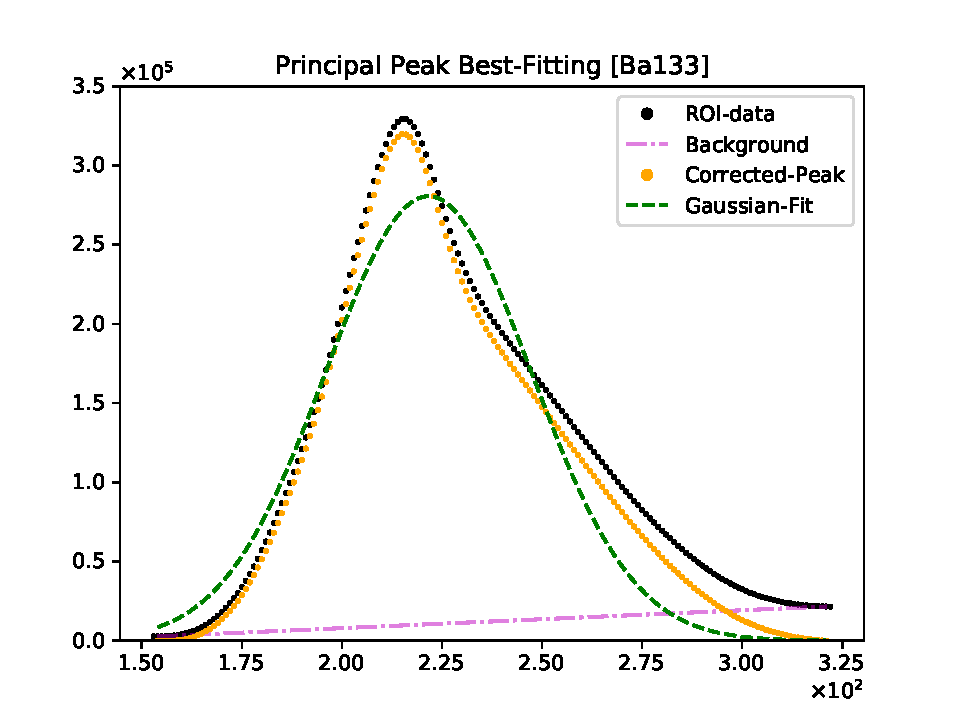
\includegraphics[width =  \textwidth,trim={1cm 0 1cm 0}, clip]{Immagini/Peak-Fitting_Ba133.pdf}
	\label{fig:PPBa133} \bigskip\bigskip
	\begin{lstlisting}[language=python, style=Pystyle, mathescape=true]
	>>> (executing file "PhytonCodeEs5.py")
	Insert the desired source [Cs137|Co57|Na22|Ba133|Eu152]: Ba133
	PRINCIPAL-PEAK POSITION 221.61534504437415 $\pm$ 1.1266699889196987
	PRINCIPAL-PEAK HEIGHT:  280582.0153386667 $\pm$ 10704.239741249454
	PRINCIPAL-PEAK WIDTH:  60.25857423710266 $\pm$ 2.6641739924518424
	PRINCIPAL-PEAK AREA : 8453736.100440461 $\pm$ 696270.7665574122
	CRYSTAL RESOLUTION:  0.27190614542073815 $\pm$ 0.013403956687680785
	\end{lstlisting}\bigskip\bigskip
\end{figure}

\newpage

\begin{figure}[h!]
	\centering
	\caption{Analisi su dati \emph{smoothed} del Picco Principale (P.P.) della sorgente Eu$^{152}$. }
	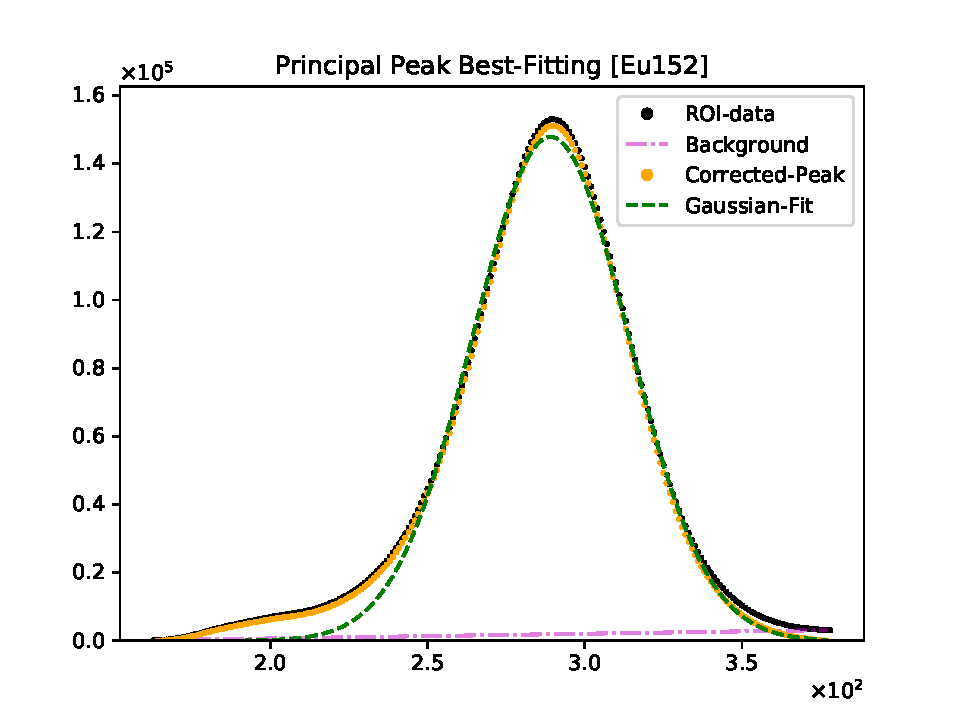
\includegraphics[width =  \textwidth,trim={1cm 0 1cm 0}, clip]{Immagini/Peak-Fitting_Eu152.pdf}
	\label{fig:PPEu152} \bigskip\bigskip
	\begin{lstlisting}[language=python, style=Pystyle, mathescape=true]
	>>> (executing file "PhytonCodeEs5.py")
	Insert the desired source [Cs137|Co57|Na22|Ba133|Eu152]: Eu152
	PRINCIPAL-PEAK POSITION 289.12654333546305 $\pm$ 0.32331257942848335
	PRINCIPAL-PEAK HEIGHT:  147846.4568358735 $\pm$ 1672.005453919737
	PRINCIPAL-PEAK WIDTH:  58.302795781850186 $\pm$ 0.7613703593365995
	PRINCIPAL-PEAK AREA : 4309930.889986031 $\pm$ 105024.2512468971
	CRYSTAL RESOLUTION:  0.20165148142141887 $\pm$ 0.002858841012675539
	\end{lstlisting}\bigskip\bigskip
\end{figure}

\newpage